\documentclass[twoside]{article}
\usepackage[utf8]{inputenc}
\usepackage[english]{babel}
\usepackage{amsmath}
\usepackage{graphicx}
\graphicspath{{./images}}
\usepackage{amsthm}
\usepackage{marvosym}
\let\marvosymLightning\Lightning
\usepackage{amssymb}
\usepackage{lastpage}
\usepackage{biblatex}
\usepackage{hyperref}
\usepackage{setspace}
\usepackage{csquotes}
\usepackage{fancyhdr}
\usepackage[dvipsnames]{xcolor}
\usepackage[framemethod=TikZ]{mdframed}
\newcommand{\R}{\mathbb{R}}
\newcommand{\Z}{\mathbb{Z}}
\newcommand{\N}{\mathbb{N}}
\newcommand{\done}{\renewcommand\qedsymbol{$\blacksquare$}}
\newcommand{\contradiction}{\renewcommand\qedsymbol{$\Lightning$}}
\usepackage[left=3cm,right=3cm,top=2cm,bottom=2cm]{geometry} % page settings
\newtheorem{lemma}{Lemma}
\newtheorem{sublemma}{Lemma}[section]
% augmented matrix environment
\newenvironment{amatrix}[1]{%
  \left[\begin{array}{@{}*{#1}{c}|c@{}}
}{%
  \end{array}\right]
}
\hypersetup{
    colorlinks=true,
    linkcolor=blue,
    filecolor=magenta,      
    urlcolor=cyan,
    pdftitle={Overleaf Example},
    pdfpagemode=FullScreen,
    }

\title{\textbf{A Swift Introduction to Group Theory}}
\author{Cade McManus, Michael Moorman}
\date{December 2022}

\addbibresource{refs.bib}

\begin{document}

% fancyhdr package header for authors' names and title
\pagestyle{fancy}
\fancyhf{}
\fancyhead[R]{\textbf{Cade McManus, Michael Moorman}}
\fancyhead[L]{\textbf{A Swift Introduction to Group Theory}}
\renewcommand{\headrulewidth}{.7pt}
\pagenumbering{arabic}
\fancyfoot[C]{\thepage\ }

\begin{spacing}{1.25}    

\maketitle

\section{Introduction}


\paragraph*{} The question ``When will I ever use this?'' is one that is likely 
most frequently asked in the math classroom and in the context of mathematics 
as a whole. This question is often difficult to answer because 
of the abstract nature of mathematics. In the context of Math 22a and linear 
algebra, this question is partially answered through the final projects 
at the end of the semester. Then, why is it that we are discussing group theory 
in this paper,
another seemingly abstract mathematical concept? The answer is that group theory
itself is a powerful tool that can be used to study the natural world in a 
mathematical, but still intuitive way. In this paper, we will explore the
fundamental ideas of group theory and how they can be applied to the real world
and other branches of mathematics,
both for the sake of understanding the world around us and for the sake of
exploring math beyond 22a for the sake of math itself. 

\paragraph*{} Throughout this paper, we will explore the basics of group theory,
how vector spaces, subspaces, and linear transformations relate to groups, and 
then examine how these ideas in group theory can be used to gain insight into 
and study all sorts of mathematical objects and spaces that have an underlying
symmetric structure to them. Group theory is very useful for studying 
these types of symmetric structures, and we seek to give the reader an intuition
for them and a basis from which to understand and study these structures. 

\paragraph*{} With this is mind, it is important to know that
our main goal is not to demonstrate some specific theorem about symmetry in its application to chemistry or something
of the sort, but rather to build the tools to approach problems like these. Therefore, many of the theorems proved
in this paper do not necessarily build towards some final
theorem, but are instead used to connect group theory to
linear algebra in a meaningful way. The effect of this
is to allow the reader to understand this new material 
because of the similarities to linear algebra that the reader ought to be familiar with already. As an example of this, Theorem 4 is not used later in the paper, but rather 
connects the idea of subgroups to subspaces of a vector space,
in order to allow the reader to meaningfully build intuition
and understanding for the idea of subgroups, rather than
simply being given the definition. 

\section{What is Group Theory?}

In order to connect the ideas of group theory to the real world, we must first understand what a group is 
in relation to linear algebra. A group is a set of elements that are closed under a binary operation,
similarly to how vector spaces are closed under addition and scalar multiplication, but with the 
generalization that groups need not be composed of only vectors, but any set of elements.

\paragraph*{Definition 1:} A \textbf{group} is a set $S$ with a binary\footnote[1]{\textbf{Binary} refers to the number of elements that the operation requires to be defined, specifically 2. Consider the binary operation of multiplication. The expression $5*$ does not make sense without a second input, making multiplication of real numbers a binary operation. }
operation $\cdot$ 
such that the following axioms hold:
% axioms of a group
\begin{enumerate}
    \item Closure: For all $a,b \in S$, $a \cdot b \in S$.
    \item Associativity: For all $a,b,c \in S$, $(a \cdot b) \cdot c = a \cdot (b \cdot c)$.
    \item Identity: There exists a unique element $e \in S$ such that for all $a \in S$, $a \cdot e = e \cdot a = a$.
    \item Inverse: For all $a \in S$, there exists a unique element $a^{-1} \in S$ such that $a \cdot a^{-1} = a^{-1} \cdot a = e$.
\end{enumerate}
Formally, the set $S$ is known as the \textbf{underlying set} of the group, and 
the binary operation $\cdot$ is known as the \textbf{group operation}. Frequently,
a group $G$ is denoted by $G = \langle S, \cdot \rangle$. Additionally, abuses 
of notation are common, such that $G$ referring to a group can be used to refer 
to the group itself or the underlying set, such that a statement like '$a\in G$'
is meant to convey that $a$ is an element in the underlying set of the group $G$.

Additionally, another special type of group we will see is an \textbf{abelian group}.

\paragraph{\textbf{Definition 2:}} An \textbf{abelian group} is a group $\langle V, \cdot \rangle$
such that for all $u,v \in V$, $u\cdot v = v\cdot u$. This means that our group operation 
is commutative, and the order in which we add elements does not matter.

\paragraph*{Example:}
This may seem confusing, but let's make it more concrete with an example: 
the real numbers together with the operation of addition as we know it. This 
group would be written $G = \langle \R, +\rangle$, and it is an abelian group. 
Let's verify our axioms 
to truly grasp what they mean through this example:
\begin{enumerate}
    \item Closure: Let $x,y\in\R$. Because the sum of any two real numbers 
    is defined as a real number, it must be the case that $x+y\in\R$. 
    \item Associativity: Let $x,y,z\in\R$. Because addition of real numbers 
    does not depend on the way in which terms are associated, it is the case 
    that $(x+y)+z = x+y+z$ and that $x+(y+z)=x+y+z$. Thus, $(x+y)+z=x+(y+z)$. 
    \item Identity: Let $e = 0$. $0\in\R$, and the addition of 0 to any $x\in\R$
    is equal to $x$ itself. Thus, for all $x\in\R$, $e+x=x+e=x$. 
    \item Inverse: For all $x\in\R$, allow $x^{-1}$, the inverse of $x$, to be equal 
    to $-x$, the negation of $x$. Thus, $-x+x=0$ via simple addition, and $e=0$.
    Therefore, for any choice of $x\in\R$, there exists an inverse element $x^{-1}$ in $\R$
    such that $x+ x^{-1} =e$, the identity element. 
    \item Commutatvitiy: Let $x,y\in\R$. Because addition of real numbers is commutative,
    it is the case that $x+y=y+x$. (Note that this case is only necessary to 
    prove that a group is abelian, not that it is a group.)
\end{enumerate}
That's all! We have proven that the real numbers, along with the operation of 
addition as we know it, form an abelian group! Now that we're a bit more comfortable with 
what a group is, what does it have to do with linear algebra? Or even anything 
else at all?

\section{Vector Spaces and their Connections to Groups}

In class, we defined a vector space as a non-empty set $V$ on which two operations,
scalar multiplication and vector addition, are defined subject to the following axioms,
where $u,v,w \in V$ and $c,d \in \R$:
\begin{enumerate}
    \item $u+v \in V$
    \item $u+v = v+u$
    \item $(u+v)+w = u+(v+w)$
    \item there exists a vector $0_v \in V$ such that $u+0_v = u$
    \item there exists a vector $-u \in V$ such that $u+(-u) = 0_v$
    \item $cu\in V$
    \item $c(u+v) = cu+cv$
    \item $(c+d)u = cu+du$
    \item $c(du) = (cd)u$
    \item $1 \cdot u = u$
\end{enumerate}
This is absolutely a correct definition, but we can introduce some additional 
notation as well as generalize $\R$. We will say that a vector space is a tuple 
$\langle V, K, +, \cdot \rangle$, where $V$ is a non-empty set, $K$ is a field\footnote[2]{A \textbf{field} refers to a set on which addition, multiplication, subtraction, etc. are defined as we know them to work for the real numbers. This is not incredibly important here, but it is relevant to note that the field $K$ is not necessarily the real numbers.},
$+$ is our vector addition operator, and $\cdot$ is our scalar multiplication operator,
and all of the previous axioms hold.

As we have seen, a group is a set of elements closed under a binary operation, which 
seems like a less restrictive version of a vector space, especially after having 
established this notation. It turns out that this is indeed the case, and that 
given our vector field $\langle V, K, +, \cdot \rangle$, we can always define 
an abelian group as simply $\langle V, + \rangle$.

\begin{mdframed}[roundcorner=10pt, backgroundcolor=gray!10]
  \textbf{Theorem 1:} Let $\langle V, K, +, \cdot \rangle$ be a vector space. Then,
  $\langle V, + \rangle$ is an abelian group.
\end{mdframed}

\begin{proof}
    In order to prove this theorem, we will verify all of the axioms of a group
    given that $V$ is a non-empty set of a vector space, and $+$ is the vector 
    addition operator from that same vector space. 
    \begin{enumerate}
      \item Closure: Let $u,v \in V$. Because axiom 1 of a vector space states that
      $u+v \in V$ and we are using the same set $V$ from our vector space and the 
      same binary operator, this property holds for our group as well.
      \item Associativity: Let $u,v,w \in V$. Because axiom 3 of a vector space states that
      $(u+v)+w = u+(v+w)$ and we are using the same set $V$ from our vector space and the
      same binary operator, this property holds for our group as well.
      \item Identity: Let $u$ be an arbitrary element of $V$. Because axiom 4 of a vector space states that
      there exists a vector $0_v \in V$ such that $u+0_v = u$ and we are using the same set $V$ from our vector space and the
      same binary operator, this property holds for our group as well using the 
      same identity element $0_v$ that we use for our vector space.
      \item Inverse: Let $u$ be an arbitrary element of $V$. Because axiom 5 of a vector space states that
      there exists a vector $-u \in V$ such that $u+(-u) = 0_v$ and we are using the same set $V$ from our vector space and the
      same binary operator, this property holds for our group as well.
    \end{enumerate}

Additionally, this is an abelian group, which requires that our group operation 
is commutative. We know that this is the case because axiom 2 of a vector space states that
$u+v = v+u$ for all $u,v \in V$, where $V$ is our underlying set and $+$ is our group operator.
Because we have shown that each of our axioms for a group holds given a non-empty 
set $V$ from a vector space and the vector addition operator $+$ from that same
vector space, and that our group operation is commutative, we have proven that
$\langle V, + \rangle$ is an abelian group formed from any arbitrary vector space 
$\langle V, K, +, \cdot \rangle$.
\done  
\end{proof}

\paragraph*{} So, there is an interesting connection between groups and vector spaces,
but the similarities and connections do not stop there. We turn to examine 
\textbf{subgroups} and their connections to vector subspaces.

\section{Subgroups}

\paragraph{} In similar fashion to the nice connection between groups and vector spaces,
there also exists an analog of subspaces in the context of groups.
\paragraph*{Definition 3:} Let $\langle G, \cdot \rangle$ be a group. Let $H$ be a non-empty subset of $G$.
We say that $H$ is a \textbf{subgroup} of $G$ if $H$ is closed under the group operation $\cdot$
and contains the identity element of $G$,
or in other words forms its own group with the binary operation $\cdot$.

\paragraph*{} Recall how we defined a subspace of a vector space in class, in 
particular that a subspace is a subset of a vector space that is closed under
scalar multiplication and vector addition and contains the zero vector.

Consider how similarly these are defined, the only difference being that 
we do not have a notion of scalar multiplication in our group. In fact, these 
are so similar that there exists a very nice continuation of Theorem 1 with 
regard to subgroups.

\begin{mdframed}[roundcorner=10pt, backgroundcolor=gray!10]
  \textbf{Theorem 2:} Let $B=\langle W,K,+,\cdot\rangle$ be a subspace of 
    vector space $A=\langle V,K,+,\cdot\rangle$. Then, $S=\langle W,+ \rangle$ is a subgroup of
    $G=\langle V,+ \rangle$.
\end{mdframed}
\begin{proof}
    In order to show this is true, we must show that $W\subseteq V$, that 
    $W$ is closed under the group operation $+$, and that $0_v\in W$, 
    all of the conditions necessary for $S$ to be a subgroup of $G$. 
    \begin{enumerate}
      \item $W\subseteq V$: This is true because $B$ is a subspace of $A$, 
      which means by definition that $W$ is a subset of $V$, the underlying set of $A$.
      \item $W$ is closed under the group operation $+$: This is true because 
      $B$ is a subspace of $A$, which means by definition that $W$ is closed under
      the vector addition operator $+$.
      \item $0_v\in W$: This is true because $B$ is a subspace of $A$, which means by definition that
        $0_v\in W$, the zero vector of $V$. By the proof of Theorem 2, we know that 
        this is the identity element of $G$ and therefore of $S$. 
    \end{enumerate}
\done     
\end{proof}

We've already shown that each vector space can be transformed into a group,
so it naturally followed already that each vector subspace can be transformed
into a group. However, now we know that these groups are subgroups of the
group formed from the original vector space! This is a very interesting result,
and further ties together the concepts of groups and vector spaces. Besides 
demonstrating these structural similarities, we can turn to examine the similarities between
functions between groups, known as \textbf{group homomorphisms}, 
and linear transformations between vector spaces.

\section{Group Homomorphisms and Isomorphisms} 

\paragraph{Definition 3:} A \textbf{group homomorphism} is a function $f:G\rightarrow H$ from a group 
$\langle G, \cdot\rangle$ to a group $\langle H, *\rangle$ such that 
$f$ preserves the group structure of $G$ and $H$. That is, $f$ must satisfy the following
property:
\begin{enumerate}
    \item $f(g\cdot h) = f(g) * f(h)$
\end{enumerate}
where $g,h\in G$.
From this property, it can be deduced that $f(e_G) = e_H$, where $e_G$ is the
identity element of $G$ and $e_H$ is the identity element of $H$, and that 
$f(g^{-1}) = (f(g))^{-1}$. We leave these proofs as an exercise to the reader.

This property may look familiar, and it should. This is exactly how we define a linear 
transformation with respect to vector addition. In fact, we can generalize this 
as follows. 

\begin{mdframed}[roundcorner=10pt, backgroundcolor=gray!10]
  \textbf{Theorem 3:} Let $\langle V, K, +, \cdot \rangle$ and
  $\langle W, L, \oplus, \odot \rangle$ be vector spaces. Then, a linear transformation
  $T:V\rightarrow W$ is a group homomorphism from $\langle V, + \rangle$ to $\langle W, \oplus \rangle$.
\end{mdframed}
\begin{proof}
One of the two axioms\footnote[3]{In class, we present this axiom as $T(u+v) = T(u) + T(v)$, but it can really be written as $T(u+v) = T(u) \oplus T(v)$, as our binary operator for vector addition may be different in our $W$ vector space.} of 
a linear transformation is that $T(u+v) = T(u) \oplus T(v)$ for all $u,v \in V$, when $T$
maps $V$ to $W$. Well, because our binary operator for our group $\langle V, + \rangle$ is $+$, and our binary operator for our group $\langle W, \oplus \rangle$ is $\oplus$, 
our sole property for a group homomorphism is satisfied simply by this one axiom 
of our linear transformation, that $T(u+v) = T(u) \oplus T(v)$ for all $u,v \in V$.
\done 
\end{proof}
Thus, group homomorphisms are generalizations of linear transformations between 
vector spaces, just like 
how groups are generalizations of vector spaces. We're not done just yet, though.
We now introduce the concept of a \textbf{group isomorphism}.

\paragraph*{Definition 4:} A \textbf{group isomorphism} is a special type of group homomorphism
that is bijective. That is, a group isomorphism is a function $f:G\rightarrow H$ from a group
$\langle G, \cdot\rangle$ to a group $\langle H, *\rangle$ such that there exists 
a function $g:H\rightarrow G$ such that $f(g(h)) = h$ and $g(f(g)) = g$ for all $h\in H$.
$g$ is known as the \textbf{inverse homomorphism} of $f$. So, a group isomorphism is a
group homomorphism that has an inverse homomorphism.

We can generalize this to linear transformations quite nicely as well.
\begin{mdframed}[roundcorner=10pt, backgroundcolor=gray!10]
  \textbf{Theorem 4:} Let $\langle V, K, +, \cdot \rangle$ and 
  $\langle W, L, \oplus, \odot \rangle$ be vector spaces. Then, a linear transformation
  $T:V\rightarrow W$ between vector spaces is a group isomorphism from $\langle V, + \rangle$ to $\langle W, \oplus \rangle$ if and only if $T$ is bijective.
\end{mdframed}

\begin{proof}
  We will prove this by showing that if $T$ is bijective, then $T$ is a group isomorphism, and that if $T$ is a group isomorphism, then $T$ is bijective.
  \begin{enumerate}
    \item If $T$ is bijective, then $T$ is a group isomorphism. 
    Let $f:V\rightarrow W$ be the function $f(v) = T(v)$ for all $v\in V$. 
    Then, $f$ is a group homomorphism from $\langle V, + \rangle$ to 
    $\langle W, \oplus \rangle$ by Theorem 3. Let $g:W\rightarrow V$ be the 
    function $g(w) = T^{-1}(w)$ for all $w\in W$. We know this 
    inverse exists because $T$ is bijective. Then, $g$ is the inverse 
    homomorphism of $f$ because $f(g(w)) = T(T^{-1}(w)) = w$ and 
    $g(f(g)) = T^{-1}(T(g)) = g$ for all $w\in W$. Thus, $T$ is a group isomorphism.

    \item If $T$ is a group isomorphism, then $T$ is bijective. 
    Let $f:V\rightarrow W$ be the function $f(v) = T(v)$ for all $v\in V$. 
    Then, $f$ is a group homomorphism from $\langle V, + \rangle$ to 
    $\langle W, \oplus \rangle$ by Theorem 3. Let $g:W\rightarrow V$ be the 
    function $g(w) = T^{-1}(w)$ for all $w\in W$. We know 
    that this inverse homomorphism exists because $T$ is a group 
    isomorphism. Then, $g$ is the inverse 
    homomorphism of $f$ because $f(g(w)) = T(T^{-1}(w)) = w$ and 
    $g(f(g)) = T^{-1}(T(g)) = g$ for all $w\in W$. Thus, $g$ is a group 
    homomorphism from $\langle W, \oplus \rangle$ to $\langle V, + \rangle$. 
    Because $f(g(w)) = w$ for all $w\in W$ and therefore $T(T^{-1}(w)) = w$ for all $w\in W$,
    we know that $T$ must be bijective\footnote[4]{
      It suffices to say that $T$ is bijective because it has a defined inverse. The 
      proof for this statement is elementary, and is left as an exercise for the reader 
      in order to keep this proof both short and on topic.
    } because it has a defined inverse for all $w\in W$.
  \end{enumerate}   
\done
\end{proof}

\paragraph*{} By now, we've laid the general groundwork for group theory. We've seen
connections to vector spaces, linear transformations, subspaces, and more. In the way
that linear algebra provides the tools to study abstract vector spaces for plenty 
of applications, the same is true for group theory. In the next section, we will see
how group theory can be used to study symmetry, in both abstract mathematical terms 
and in the context of physical systems! 

\section{Groups of Functions, Symmetry, and Group Actions}
\paragraph*{} We have seen how vector spaces can satisfy the group axioms, so a natural 
area of inquiry might be to dig further into the connection between these objects. 
For example, instead of investigating questions about groups directly, might we instead 
be able to study some equivalent vector space / linear algebraic object and then leverage 
the tools that we have been studying this semester to answer our original question? As 
it turns out this is indeed possible. For the purposes of this paper (and simplicity) 
feel free to assume the relevant objects are finite linear groups. 

\paragraph*{} To find the explicit connection we will first introduce the notion of 
\textbf{group actions} in the context of vector spaces. Suppose we have a real vector space 
$V=\langle \R^n,K,+,\cdot\rangle$, and the 
set of $n$ x $n$ invertible matrices\footnote[5]{Typically, $M_{n\text{x}n}$ denotes the set of all $n$x$n$ matrices, but we will
use this notation to denote the set of invertible matrices for simplicity 
and because we will not use non-invertible matrices in this paper.
}, $M_{n\text{x}n}$, in that space.
This set of matrices is known as the \textbf{general linear group} of $V$, GL($V$),
and is indeed a group under matrix multiplication as the binary operator.
\begin{mdframed}[roundcorner=10pt, backgroundcolor=gray!10]
  \textbf{Theorem 5:} The set of $n$ x $n$ invertible matrices, $M_{n\text{x}n}$, in
  $\R^n$ forms a group under matrix multiplication as the binary operator, written 
  $\langle M_{n\text{x}n}, \circ\rangle$.
\end{mdframed}
\begin{proof}
  We will prove this by showing that $M_{n\text{x}n}$ is closed under matrix multiplication, 
  that the identity matrix is an identity element, and that the inverse of a matrix is 
  indeed its inverse. 
  \begin{enumerate}
    \item $M_{n\text{x}n}$ is closed under matrix multiplication. 
    Let $A,B\in M_{n\text{x}n}$. Then, $A$ and $B$ are invertible $n$ x $n$ matrices. 
    Then, det$(A) \neq 0$ and det$(B) \neq 0$ by the IMT. Because det($AB$)=det$(A)$det$(B)$,
    we know that the matrix $AB$ does not have a zero determinant, so it is invertible.
    Then, $AB\in M_{n\text{x}n}$.

    \item The identity matrix is an identity element. 
    Let $A\in M_{n\text{x}n}$. Because $AI_n=A$ and $I_nA=A$, we know that $I_n$
    is an identity element for $M_{n\text{x}n}$. 

    \item The inverse of a matrix is its inverse group element.  
    Let $A\in M_{n\text{x}n}$. Then, $A$ is an invertible $n$ x $n$ matrix. 
    Then, $A^{-1}$ is also an invertible $n$ x $n$ matrix. Because $AA^{-1}=I_n$,
    we know that for all $A\in M_{n\text{x}n}$ there exists an $A^{-1}$ such that $AA^{-1}=I_n$.
  \end{enumerate}
  Thus, $M_{n\text{x}n}$ is a group under matrix multiplication as the binary operator.
\done 
\end{proof}

\paragraph*{} This may seem trivial, but recognize how this is different from our 
previous examples of groups. Matrices as we know them are not only objects, 
but linear transformations themselves. This opens the door for not only studying 
groups of objects like vectors, but also for bijective functions, in this example 
over vector spaces. Additionally, consider that matrix multiplication is simply 
the composition of matrices. Thus, we can think of the group of matrices as a
group of functions (linear transformations), with the binary operator of 
function composition over a certain domain. 

\paragraph*{} With it in mind that groups can take the form of sets of functions 
and transformations over vector spaces, consider how we could extend this to 
other domains besides vector spaces. Additionally, consider how these matrices 
are all invertible, and preserve the structure of the vector space. This is an 
important property, and is highly related to the notion of symmetry when 
groups like these are extended to physical systems. 

\paragraph*{} This idea is important, so consider the example of
a square (consider the location of its vertices, sides, or any defining property
to be our domain). If you were to rotate that square by 90 degrees, it would look exactly the 
same. Its vertices may be in different locations, but they were mapped to each other 
in a such a way that the structure we care about preserving (square-ness) is kept 
intact. Also, notice that there are many different symmetries that one could exploit 
to perform a symmetric action, such as flipping the square over. 
We've kept things intuitive so far, but lets make our terminology a bit more precise.

\paragraph*{Definition 5:} A \textbf{symmetry operation} on some object $X$ is an automorphism, that is, an ismorphism  $\beta: X \rightarrow X$.
\begin{mdframed}[roundcorner=10pt, backgroundcolor=gray!10]
  \textbf{Theorem 6:} Let Sym($X$) be the set of symmetry operations of $X$, then Sym($X$) under composition is a 
  \textbf{symmetric group}.
\end{mdframed}
\begin{proof}
Associativity: In \textit{How to Prove it, a Structured Approach} on page 176 they show that function composition
is always associative. This is a known result and we leave its verification to the reader.\\
Identity: We let our identity operation be the automorphism that maps every element of $X$ to itself, and denote this
$e$. Then for arbitrary $g \in \text{Sym}(X), (g \circ e)(X) = g(x)$, as doing nothing to $X$ and then applying $g$
should be exactly the same as just applying $g$.  \\
Inverses: By the definition of symmetry operation, for all $g \in \text{Sym}(X)$, $g$ is a bijective endomorphism (map from $X$ to itself), which means its inverse operation exists and is also an element in Sym($X$). Thus
$(g \circ g^{-1})(x) = e(x)$ as applying a function, and then undoing the function is the same as doing nothing.\\
Closure: We will show closure by showing that composition of arbitrary elements of Sym($X$), $g, h \in \text{Sym}(X)$
must also be an automorphism from $X$ to $X$. As $g$ and $h$ map $X$ to itself, their composition must also do this, so 
$g \circ h$ is an endomorphism from $X$ to $X$. We also know this endomorphism is bijective as we have inverse composition $h^{-1} \circ g^{-1}$ such that $ (h^{-1} \circ g^{-1})(g \circ h)(x) = x$ for all $x \in X$. Thus we find
that every composition is an automorphism, and thus also an element of Sym($X$). \\
As all group conditions are satisfied, the set of automorphisms of object $X$ form a group.
\done 
\end{proof}

\paragraph*{Definition 6:} A \textbf{symmetry group} of an object $X$ is a
group $G$ of transformations of $X$ that preserves the structure of $X$ with 
the binary operator of composition. It is commonly denoted as $G=\text{Sym}(X)$.

\paragraph*{} The upshot is this: groups have a deep connection to symmetry, and 
\textbf{group actions} acting on a set are homomorphisms from a given group into
the group of transformations of that set. 
When we can perform group actions on a vector space $V$, we 
can often map group elements to subgroups of GL($V$), allowing us to use linear algebra.
We now formalize what we mean by a `group action'.

\paragraph{\textbf{Definition 7:}} If $G$ is a group with identity element
$\epsilon$ and $X$ is a set, then a function \\ $\alpha: G \times X  \rightarrow X$
is a \textbf{group action} if it satisfies the following two axioms:
 \begin{enumerate}
  \item $\text{Identity:} \: \alpha(\epsilon, x) = x \text{ for all } x \in X$ 
  \item  $\text{Compatability:} \: \alpha(g, \alpha(h,x)) = \alpha(gh, x) \text{ for all } x \in X$
 \end{enumerate}


\paragraph*{} Remember that we have 3 objects under consideration. A group $G$ with some underlying set, a set $X$, and the symmetry group of $X$, $\text{Sym}(X)$. Elements in $G$ can be mapped via the
group action injectively but not necessarily surjectively into $\text{Sym}(X)$, however, if we 
look only at the subgroup formed by the range of $\alpha$ then $\alpha$ is an ismorphism.
We interpret $\alpha(g, x)\: 
(\text{where} \: g \in G, x \in X)$ as first mapping g to some symmetry operation of $X$, and then
mapping x according to that symmetry operation. Back in the 
square example, $X$ would be  the set of vertices, $x$ would be the top right vertex, and 
$g$ would be mapped to, for example, the symmetry operation of $\ 90^{\circ}$ clockwise rotation, and 
$\alpha(g, x)$ would output the bottom right vertex.

% reference for Cayley's theorem?
\paragraph*{} While the linear case of group actions may not always apply, 
Cayley's theorem tells us that every group is isomorphic to a subgroup of some 
symmetric group.

\begin{mdframed}[roundcorner=10pt, backgroundcolor=gray!10]
    \textbf{Theorem 7:} Every group is \textbf{isomorphic} to a subgroup of a \textbf{symmetric group}.
\end{mdframed}
\begin{proof}
Suppose group $\langle G, * \rangle$, the set of permutations of $G, P = \{\lambda_g:G \rightarrow G : g \in G\}$ 
where $\lambda_g(x) = g * x$, and the map $\rho:G \rightarrow P$. We will prove the P is a symmetry group under composition, and then that $\rho$ is a homomorphism and is also bijective. \\
Sub Claim: P is a symmetry group \\
Injectivity: For arbitrary $g \in G$, suppose $\lambda_g(x) = \lambda_g(y)$. Then $g * x = g * y$. As G is a group we can
left multiply by $g^{-1}$ and find that $g^{-1} * g * x = g^{-1} * g * y \rightarrow x = y$, so $\lambda$ is injective.
Surjectivity: Suppose arbitrary $g, h \in G$. As G is a group we know $(g^{-1} * h) \in G$, so
$\lambda_g(g^{-1}*h) = g * g^{-1} * h = h$, so for an arbitrary element in the codomain of $\lambda_g$ there is an 
element in the domain that is mapped to it, so $\lambda$ is surjective. \\
As the $\lambda_g$ is injective and surjective it is also bijective. As $g$ was arbitrary all elements of P are
bijective. Then $P$ is the set of symmetry operations of $G$, so $P$ = Sym($G$), which by our earlier theorem form a 
symmetric group under composition. \\
\textbf{Lemma:} $\rho$ is a homomophism that is bijective. \\
Homomorphism: \begin{equation}
    \rho(g * h)(x) = \lambda_{g * h}(x) = g * (h * x) = \lambda_g(h * x) = (\lambda_g \circ \lambda_h)(x) =
    (\rho(g)\circ\rho(h))(x)
\end{equation} \\
Surjectivity: For arbitrary $\lambda_g$, $\rho(g) = \lambda_g$, so the function is surjective. \\
Injective: Suppose $\lambda_g(x) = \lambda_h(x)$. Then for all $x \in G$ then functions are equal, in particular,
$\lambda_g(e) = \lambda_h(e) \rightarrow g*e = h*e \rightarrow g = h$. So the function is injective. \\
As $\rho$ is surjective, injective, and a group homomorphism, it is an isomorphism to a symmetric group,
as required.
\done
\end{proof}

\section{Representations}
\paragraph*{} Now that we have done the groundwork we are ready to make 
explicit this intuitive connection between groups and vector spaces using 
\textbf{Representation Theory}. A \textbf{representation} is a group action onto GL($V$), 
where $V$ is a vector space. The elements of a group are mapped to invertible 
matrices in this case. 

\textbf{Definition 8:} A \textbf{representation} of group $G$ on a vector space 
$V$ over field $K$ is a group homomorphism $\rho: G \rightarrow GL(V)$ 
such that $\rho(g, h) = \rho(gh)$ for $g,h\in G$.

\paragraph*{} We've been a bit abstract, so let's look at an example of a group, 
and show how one might generate such a representation. Lets consider an equilateral 
triangle as our object, and its corners the elements we are tracking. It turns out 
that there are 6 symmetry operations (including the do-nothing identity) we can 
perform to leave the triangle looking the same. For now, consider the 
clockwise ${120}^{\circ}$ rotation, denoted as $q$. This is notational abuse, as given 
our previous description, $q$ should be an element of a group we are mapping to the 
set of symmetry operations. 
% make clear why we use this abuse of notation
In any case, we want to find an invertible matrix 
that captures what this element $q$ does. That ought to sound familiar. When we wanted 
to find a matrix for a linear transformation, we looked at where it took our basis 
vectors - so let's choose a basis corresponding to the elements we are tracking. 
Let $t$, $l$, $r$ correspond to the top, left, and right vertex respectively. 
\[
t = 
\begin{bmatrix}
1 \\
0 \\
0 \\
\end{bmatrix}, \;
l = 
\begin{bmatrix}
0 \\
1 \\
0 \\
\end{bmatrix}, \;
r = 
\begin{bmatrix}
0 \\
0 \\
1 \\
\end{bmatrix}
\] 
\paragraph*{}  Note that the standard basis was chosen merely for convenience, 
and any basis could function equivalently (this will come up a bit later). These vectors would look like this in $\R^3$:
\begin{center}
  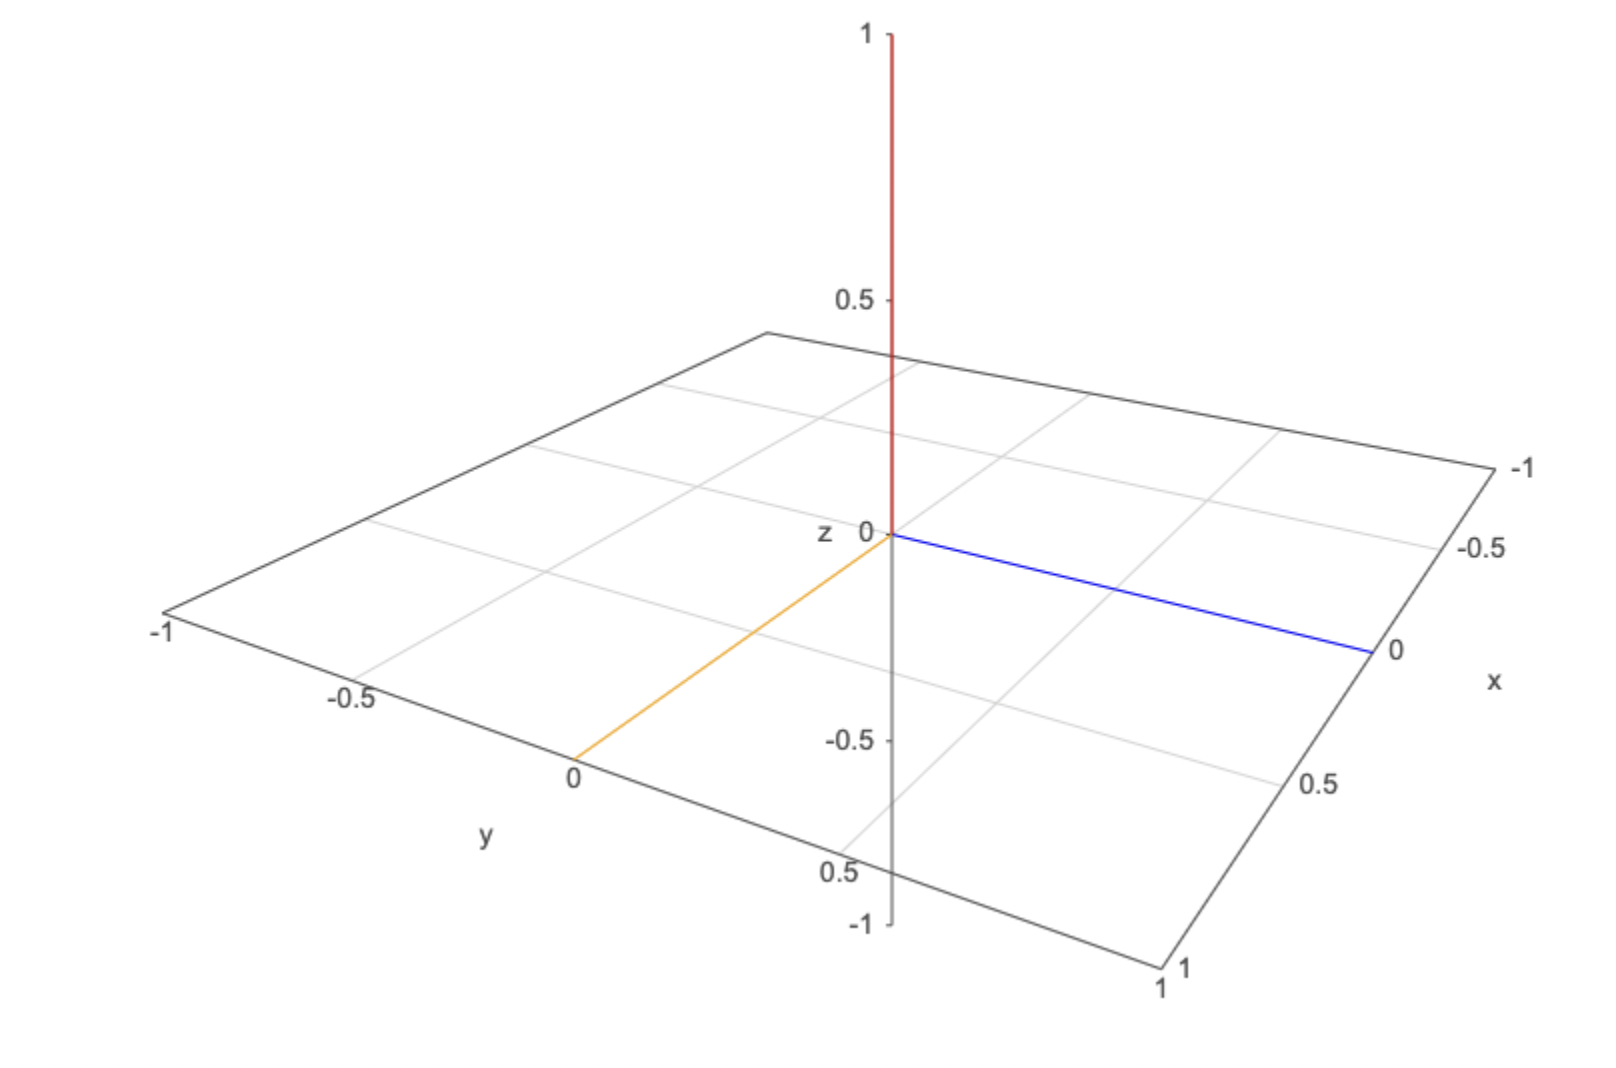
\includegraphics[scale=0.35]{images/first.png}  
\end{center}
    
Now let's observe where $q \cdot t$, $q\cdot l$, and $q \cdot r$ take our basis vectors. As a 
reminder, $q$ is a ${120}^{\circ}$. rotation. For simplicity sake we shorten 
$\rho(q, x)\: \text{to} \: q \cdot x$.
\[
q \cdot t = 
\begin{bmatrix}
0 \\
0 \\
1 \\
\end{bmatrix}, \;
q \cdot l = 
\begin{bmatrix}
1 \\
0 \\
0 \\
\end{bmatrix}, \;
q \cdot r = 
\begin{bmatrix}
0 \\
1 \\
0 \\
\end{bmatrix}
\]

These can be visualized as well, and by tracking the colors, it can be seen that these vectors have each moved, completing a 120 degree rotation of the resultant triangle formed from their endpoints when drawn from the origin. 

\begin{center}
  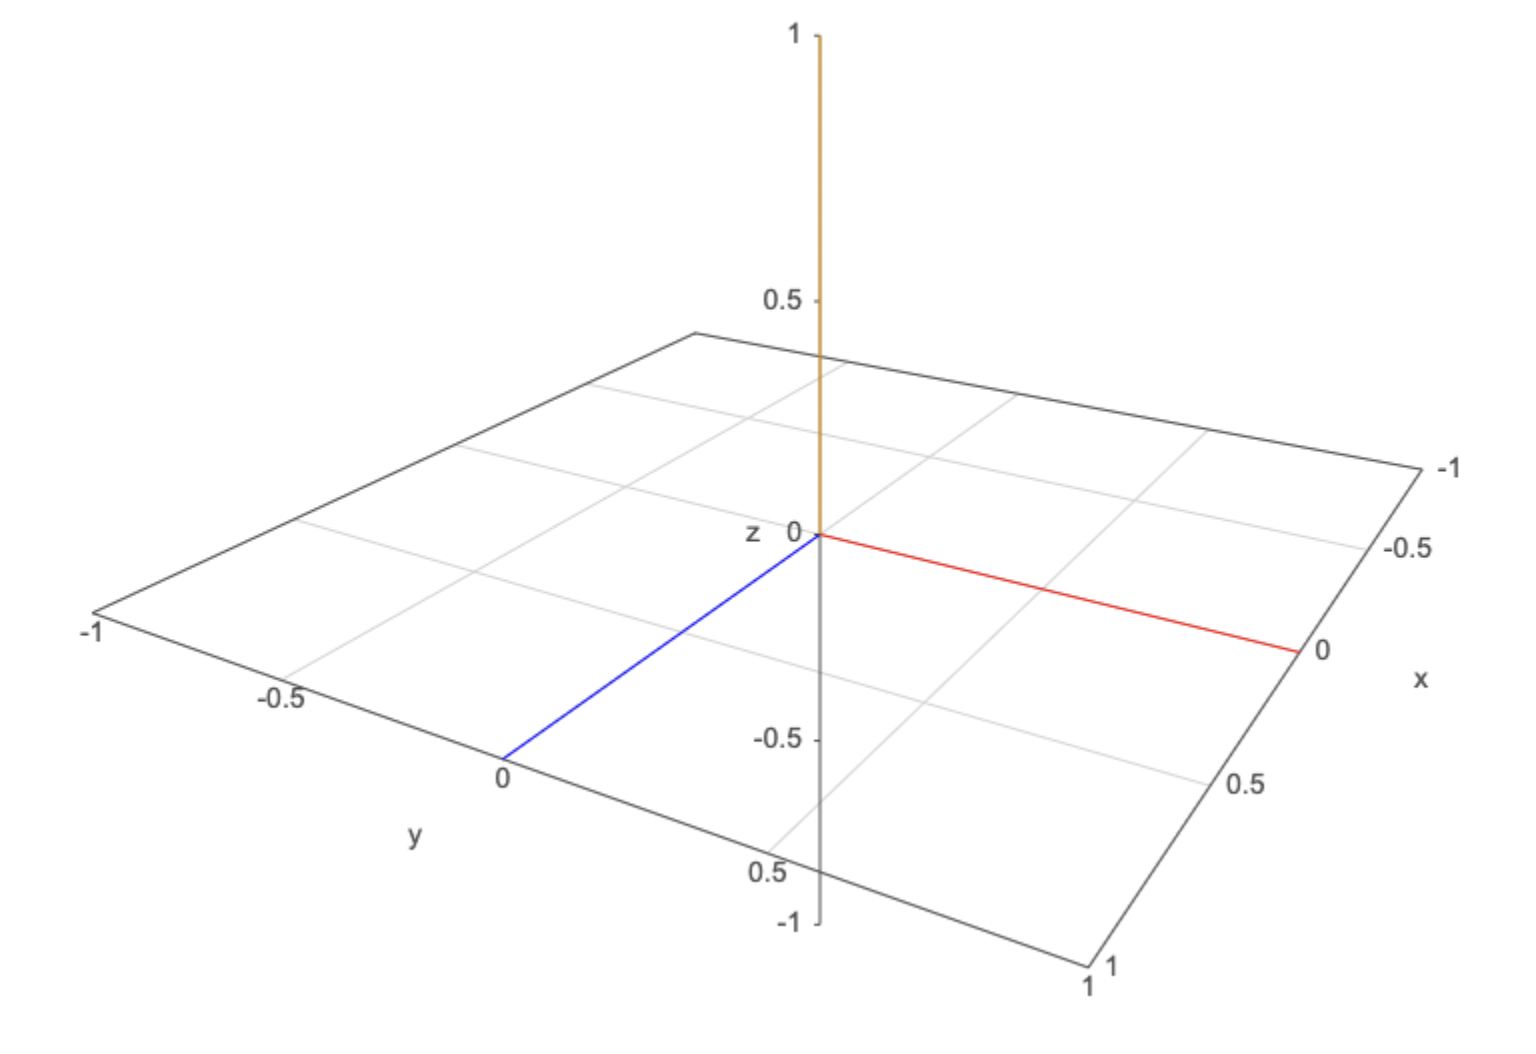
\includegraphics[scale=0.35]{images/second.png}  
\end{center}

\paragraph*{} So, just as we have done in class we can, with respect to our chosen basis, write an explicit matrix for $q$.
\[
q = 
\begin{bmatrix}
0 & 1 & 0 \\ 
0 & 0 & 1 \\
1 & 0 & 0 \\
\end{bmatrix}
\]

\paragraph*{}  This sort of representation may seem specific,
but consider how many different symmetrical operations this method could represent. For example, could you come up with some way to represent the operation of flipping the triangle 
in some way?

You might have noticed that a different choice of basis could lead to significantly different
representations for the same operations. Intuitively, though, choosing a different basis shouldn't
change anything fundamental about the information we want our representation to hold. We've encountered a similar problem in class, when our linear transformations
looked quite different upon first inspection, but actually could be connected with just a change of basis. A similar idea can be applied here.
\paragraph{Definition 9:} A \textbf{homomorphism} between two representations ($\lambda_w, W)$ and $(\lambda_v, V)$ under group G, is the map
 $\lambda:V \rightarrow W$ where 
$\lambda\circ\lambda_v(g) = \lambda_w(g)\circ\lambda$ for all.
\paragraph{Definition 10:} Two representations are \textbf{isomorphic} if there is an invertible representation homomorphism $\lambda:V \rightarrow W$
, such that $\lambda_v = \lambda^{-1}\circ\lambda_w\circ\lambda$

\paragraph{}So as it turns out, our change of basis is irrelevant up to isomorphism between representations! Now, this only scratches 
the surface of representation theory (and its nice connections to our classwork), but given the scope of this paper lets pause here and briefly look at some 
real life applications of representation theory.

\paragraph{} A classic application of group theory in the real world is in chemistry, through something called
Molecular Orbital theory. Roughly speaking, the problem at hand is predicting the properties of molecules
without directly performing experiments. This is especially hard when molecules oscillate between many structures. As it turns out, these oscillations are "symmetry preserving" and also often change properties of the molecules in
predictable ways, and can thus be modeled as group actions.
Then, they can be meaningfully modeled by representations 
as matrices, which allows the properties of these oscillations to be easily studied and understood, as well
as simulated easily by a computer. 

\section{Conclusion}

\paragraph*{}  In this paper we have shown that groups are intimately related to
vector spaces, and that this relationship can be made explicit using representation
theory. We have also shown that the notion of irreducible representations is a
useful tool for understanding the structure of groups. 

With the study of linear algebra and abstract vector spaces, we have seen 
in class how it can be applied to many different scenarios where the generalizations 
linear algebra provides can be extremely useful. This is also the case for 
the extension of group theory and representation theory. Not only can we study 
symmetric structures using group theory, but we can also apply what we've learned 
throughout this semester in linear algebra to these structures. While this paper 
may have been a bit abstract, the hope is that it has given the reader the basic 
tools to approach all sorts of future problems, whether abstract or concrete. 

\paragraph*{} Additionally, for those interested in how Rubik's cubes relate to group theory, an interesting 
(but sufficiently challenging) paper written by Harvard's own Janet Chen can be found
\href{https://people.math.harvard.edu/~jjchen/docs/Group%20Theory%20and%20the%20Rubik's%20Cube.pdf}{here}.


\newpage

\nocite{*}
\printbibliography
\end{spacing}

\end{document}
